\documentclass[a1paper,portrait,fontscale=0.43]{baposter}

\columnsep=70pt % This is the amount of white space between the columns in the poster
\columnseprule=3pt % This is the thickness of the black line between the columns in the poster

\usepackage{multicol} % Required for multiple columns
\setlength{\columnsep}{1.5em} % Slightly increase the space between columns
\setlength{\columnseprule}{0mm} % No horizontal rule between columns
\setlength{\multicolsep}{0mm} % No horizontal rule between columns

\usepackage[font=small,labelfont=bf]{caption}

\usepackage{wrapfig}
\usepackage{lmodern}

\usepackage[utf8]{inputenc} %unicode support
\usepackage[T1]{fontenc}

\selectcolormodel{cmyk}

\graphicspath{{figures/}{../../schematics/svg/}} % Directory in which figures are stored

\newcommand{\compresslist}{%
  \setlength{\itemsep}{0pt}%
  \setlength{\parskip}{1pt}%
  \setlength{\parsep}{0pt}%
}

\newenvironment{boenumerate}
  {\begin{enumerate}\renewcommand\labelenumi{\textbf\theenumi.}}
  {\end{enumerate}}

\begin{document}

\definecolor{darkgreen}{cmyk}{0,0.90,0.74,0.28}
\definecolor{lightgreen}{cmyk}{0,0.90,0.74,0.28}
\definecolor{chartreuse(web)}{rgb}{0.5, 1.0, 0.1}

\begin{poster}
{
grid=false,
headerborder=open, % Adds a border around the header of content boxes
colspacing=1em, % Column spacing
bgColorOne=white, % Background color for the gradient on the left side of the poster
bgColorTwo=white, % Background color for the gradient on the right side of the poster
borderColor=black, % Border color
headerColorOne=chartreuse(web), % Background color for the header in the content boxes (left side)
headerColorTwo=lightgreen, % Background color for the header in the content boxes (right side)
headerFontColor=white, % Text color for the header text in the content boxes
boxColorOne=white, % Background color of the content boxes
textborder=roundedleft, %rectangle, % Format of the border around content boxes, can be: none, bars, coils, triangles, rectangle, rounded, roundedsmall, roundedright or faded
eyecatcher=false, % Set to false for ignoring the left logo in the title and move the title left
headerheight=0.18\textheight, % Height of the header
headershape=rounded, % Specify the rounded corner in the content box headers, can be: rectangle, small-rounded, roundedright, roundedleft or rounded
headershade=plain,
headerfont=\Large\bf\textsf, % Large, bold and sans serif font in the headers of content boxes
%textfont={\setlength{\parindent}{1.5em}}, % Uncomment for paragraph indentation
linewidth=2pt % Width of the border lines around content boxes
}
{}
%
%----------------------------------------------------------------------------------------
%	TITLE AND AUTHOR NAME
%----------------------------------------------------------------------------------------
%
{  
  {
\includegraphics[trim=1.7cm 0 0 0.5cm, width=247mm]{DSP-02}\vspace{0.5em}}% SASE logo


  \bf\textsf %Sans Serif  
  {Dynamic Reuse of Memory in 2D Convolution Applied to Image Processing}
} % Poster title
% {\vspace{1em} Marta Stepniewska, Pawel Siedlecki\\ % Author names
% {\small \vspace{0.7em} Department of Bioinformatics, Institute of Biochemistry and Biophysics, PAS, Warsaw, Pawinskiego 5a}} % Author email addresses
{{\sf\vspace{0.2em}\\
    Martin Casabella,
    Sergio Sulca,
    Ivan Vignolles,
    Ariel L. Pola
\vspace{0.2em}\\
\small{Department of Research and Development Fundacion Fulgor 
\vspace{0.2em}\\
martin.casabella@gmail.com, ser.0090@gmail.com,
    ivanmvig@gmail.com and arielpola@gmail.com}
}}
%{
\includegraphics[width=0.1\textwidth]{logo}} % University/lab logo

\headerbox{1. Introduction}{name=introduction,column=0,row=0, span=3}{
\footnotesize{
%The origin of digital image processing is directly related to the development and evolution of computers. Most
%image filters that focus, blur, enhance edges and detect edges, among
%others, use convolution as a mathematical operation. Image processing is a very
%extensive research area with a large number of applications in multiple fields
%such as medicine, engineering, navigation, aeronautics, among others.
%Convolutional neural networks (CNN)~\cite{Lecun-et-al-1998} have received
%increasing attention in recent years. This technique uses a fast and efficient
%convolution implementation.
%
The implementation of high-speed image processing systems in field programmable
gate array (FPGA) has been a very active field. This is mainly due to the
ability to take advantage of bit level parallelism, pixel level, neighborhood
level and task level to increase computing performance and speed. %In addition, FPGAs are
%reconfigurable, allowing the flexibility that is often desired in neural
%networks. This combination of parallel processing and flexibility at very high
%speed, is what makes FPGAs a platform of choice for the development of these
%areas~\cite{papercnn}.

There are many examples in the literature of two-dimensional (2D) convolution
implementations, where most of the work focuses on high performance, resource
reduction and FPGA area efficiency. As shown in~\cite{paper3}, block random access
memory (BRAM) is one of the most used elements with the highest energy
consumption. Therefore, the architectures seek to reduce the use of BRAMs by
dividing them into two groups that consider either total storage or partial storage of the
image. The first of them increases processing by applying parallelization as
well as reusing resources to reduce complexity~\cite{paper1,paper5}. On the
other hand, architectures with partial storage partition the image into as many
parts as convolders are used~\cite{paper2,paper4}. The drawback presented by
these schemes is the non-modularization of processing, making it difficult to
improve the work rate by increasing parallelism.

In this work, we explain the concept of dynamic reuse of BRAM in 2D convolution
and its complexity concerning implementation for parallel architectures. Moreover, we
propose a modular architecture, where it is easy to appreciate that when the
parallelism level increases, the complexity of BRAM increases linearly.

%This paper is organized as follows. Section~\ref{sec:preproc} introduces the
%image processing algorithm. The archicterure design is
%presented in section~\ref{sec:architecture}. In
%section~\ref{sec:implementation}, hardware implementation and experimental
%results are shown. Finally, conclusions are drawn in
%section~\ref{sec:conclusion}.
}}


\headerbox{2. Image Processing}{name=model,column=0,below=introduction,span=1}{
%Python was the programming language utilised for all data and model analysis, and application development purposes. Some third-party libraries used in this experiment were: PyQt5, numpy, pandas, pickle, scikit-learn, xgboost, lightgbm, rgf, elm, keras and tensorflow.\\
%
%All data was cleaned accordingly prior evaluation. Furthermore, by using cross-validation techniques, the data was split up into training and testing sets. The training of all models by fitting the training sets (all data split into partitions by cross-validation) was then followed by fitting the testing features to obtain a prediction set. In turn, by utilising these predictions for evaluation, some scoring metrics resulted for comparison.
%\begin{center}
%    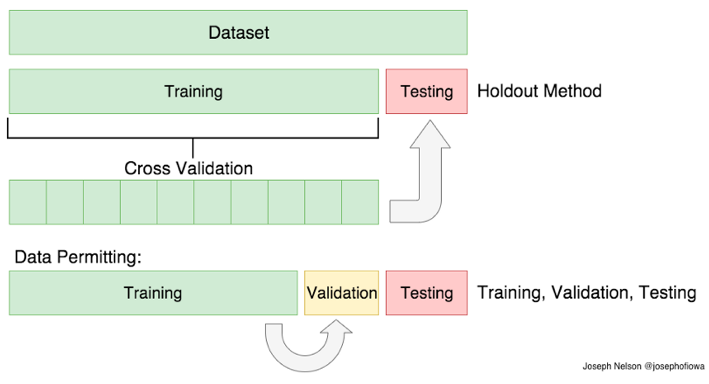
\includegraphics[width=\linewidth]{cv}
%\end{center}

%\begin{center}
%    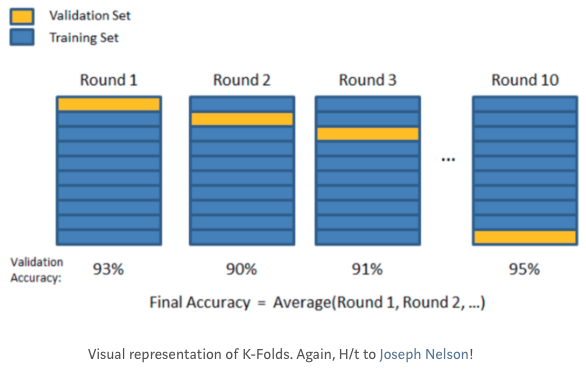
\includegraphics[width=\linewidth]{kfoldrep}
%  \end{center}
Given its local and two dimensional nature, 2-D Convolution is one of the most used image processing algorithms. 
Inherent parallelism of the image convolution algorithm can be exploited to increase the performance.
We focus our study on a more efficient design of 2D convolution technique
to reduce the usage of  FPGA resources.% So the images used for processing are grayscale. %because of its implementation simplicity, but the design can be extrapolated
%to multiple channel images by considering each channel as an independent grayscale image.

The pixels of grayscale images $I(x,y)$ have a dynamic range between
$[0,255]$ and Kernel values $K(x,y)$ can be negative or positive. This work is
part of a Deep Learning project where it is usual to operate with a dynamic
range centered on zero. Therefore, we apply dynamic range expansion
$(\mathcal{D}[.])$~\cite{dinamic_rango} and maximum norm
$(\mathcal{M}[.])$~\cite{max_norm} to rearrange
$\mathcal{D}[I(x,y)]=I^\prime(x,y)$ between $[0,1]$ and
$\mathcal{M}[K(x,y)]=K^\prime(x,y)$ between $[-1,1]$, respectively
Therefore, replacing in bidimensional convolution formula 
 $$G(x,y) = \mathcal{D}^{-1}\left[\sum_{i=0}^{m-1} \sum_{j=0}^{n-1}K^\prime(i,j)I^\prime(x-i,y-j)\right],$$ 
Where $\mathcal{D}^{-1}[.]$ is the dynamic range change between $[0,255]$ in the
FPGA. Finally, all the processed blocks are reordered by software.
\begin{center}
  
\includegraphics[width=\linewidth]{wflow3}
\end{center}
}

\headerbox{3. Architecture Design}{name=screen,span=2,column=1,below=introduction}{ % To reduce this block to 1 column width, remove 'span=2'


%At every fold during the cross-validation process, each model returns a set of predictions, which the application stores. At the end of all iterations (10 iterations, since the cross-validation method implemented, is tuned to partition the data in 10 folds), the mean for every performance metric and each executed algorithm was calculated.

%\hspace{0pt}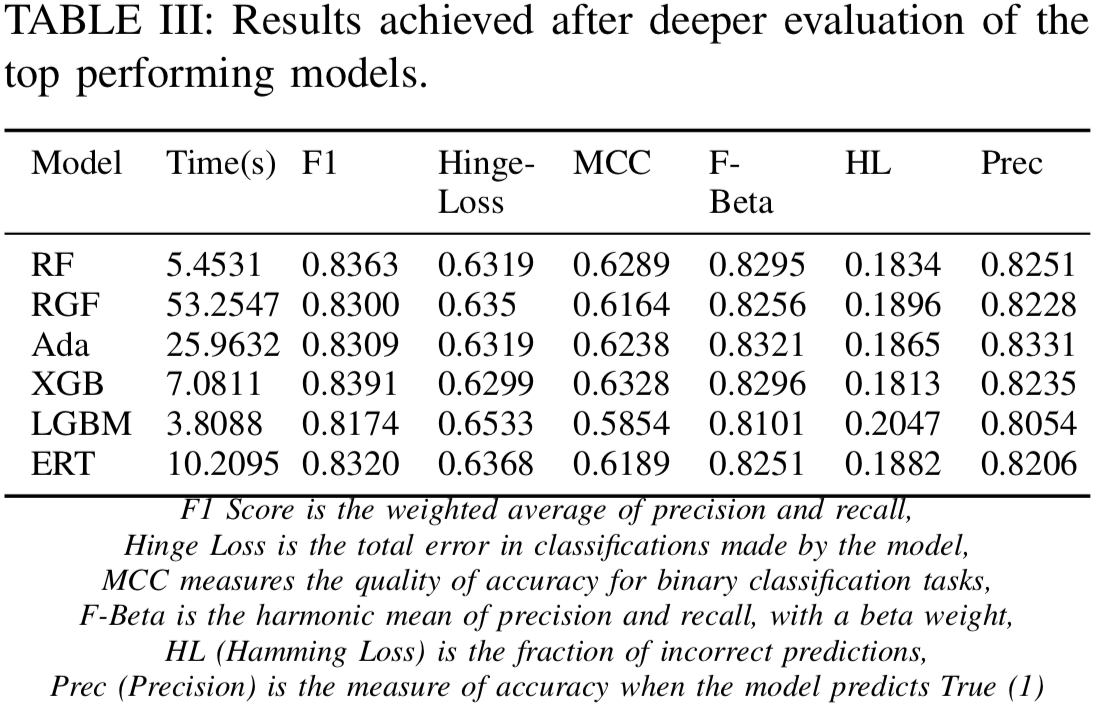
\includegraphics[width=\linewidth]{r2}

\begin{multicols}{2}
    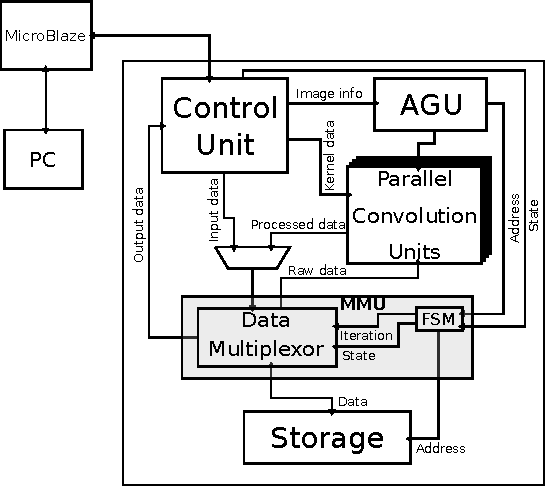
\includegraphics[width=\linewidth]{general}
\vfill\null
\columnbreak
The pre-processing consists of capturing the image and applying
the transformation using a Python script. In addition, the script divides the
image into batches and sends them through the UART port to the FPGA. A batch
consists of contiguous pixel columns. In the FPGA a microprocessor receives the
information and transfers it to the convolution module using a 32 bits general
purpose input-output (GPIO) port. The second stage is the processing. The batch is convolved with the kernel inside
the module, which is established by the user through the GPIO.
The \textbf{control unit} is the one in charge of handling the communication with
the processor and the \textbf{multiplier-accumulator (MAC) unit} executes the sum
of the products of the kernel's coefficients with the pixels. The \textbf{address generation unit (AGU)}
\end{multicols}
manages the memory addresses along with
the \textbf{memory management unit (MMU)}, that decides how the values in memory
are read and written.
The last module is the \textbf{storage} one, which is
implemented with a set of columns of the FPGA's block RAM. 

When the operation ends, a notification is sent to the microprocessor,
which gives the order to recover the processed batch from the module and sends it
to the central processing unit (CPU). Finally, the post-processing stage combines
the batches on the CPU using a Python script.
}

\headerbox{4. Implementation and Results}{name=sea,span=2,column=1,below=screen}{ % To reduce this block to 1 column width, remove 'span=2'

\begin{multicols}{2}

The design was implemented in a Xilinx Artix-35T FPGA (xc7a35ticsg324-1L) using
Xilinx Vivado Design Suite 2017.4 tools. A $100$ MHz reference clock
was synthesized.

Considering only convolution operation processing, i.e. not taking into account
the time needed to load the image into memory, one pixel per clock cycle ($100$ Mhz) is
obtained per instantiated MAC unit. Thus, throughput increases linearly with
parallelism degree. Table \ref{conv_tp} shows throughput obtained for
different parallelism degrees.
The architecture was synthesized for different degrees of parallelism.
Table~\ref{res_table} shows module and microprocessor complexity
on the FPGA with and without DSP respectively, measured by resource utilization. As a result, a linear increase is
shown according to parallelism. Due to implemented FPGA limitations a
parallelism up to 8 was achieved using DSP and up to 24 without DSP but with a
more intensive LUT usage.


\begin{center}
\begin{tabular}{|c|c|c|}
\hline
\textbf{Parallelism}  &    \textbf{Processing Speed [Mp/s]}  \\ \hline
        2             &                     200              \\ \hline
        4             &                     400              \\ \hline
        8             &                     800              \\ \hline
\end{tabular}           
\captionof{table}{Throughput achieved in convolution processing.}
\label{conv_tp}
\end{center}

\end{multicols}
\begin{center}
\begin{tabular}{|c|c|c|c|c|c|c|}
  \hline
  & \multicolumn{3}{c|}{\textbf{With DSP [N](\%)}} & \multicolumn{3}{c|}{\textbf{Without DSP [N](\%)}} \\ \hline
  \textbf{P}  & \textbf{DSP}            & \textbf{LUT}        & \textbf{BRAM}       & \textbf{DSP}         & \textbf{LUT}           & \textbf{BRAM}         \\ \hline
  2  & 20(22)         & 1845(9)    & 10(20)     & ---         & 3168(15)      & 10(20)         \\ \hline
  4  & 40(44)         & 2022(10)   & 11(22)     & ---         & 4627(22)      & 11(22)         \\ \hline
  6  & 60(67)         & 2175(10)   & 12(24)     & ---         & 6063(29)      & 12(24)         \\ \hline
  8  & 80(89)         & 2448(12)   & 13(26)     & ---         & 7756(37)      & 13(26)         \\ \hline
  10 & ---            & ---        & ---        & ---         & 9328(45)      & 14(28)         \\ \hline
  12 & ---            & ---        & ---        & ---         & 10917(52)     & 15(30)         \\ \hline
  24 & ---            & ---        & ---        & ---         & 20209(97)     & 21(42)         \\ \hline
\end{tabular}           
\captionof{table}{Resource utilization table with and without DSP.}
\label{res_table}
\end{center}
}
	
\headerbox{5. Conclusions}{name=conclusion,column=1,below=sea,span=2,above=bottom}{
\footnotesize{
% DeCAF is a chemoinformatical tool that can be helpful in ligand-based drug design.
% It provides a comprehensive molecule description and a fast algorithms for comparing and aligning multiple ligands.
%This research proves that Random Forests and the boosting methods LightGBM and XGBoost are amongst of the most highly effective techniques to predict and classify players as either exhibiting problematic behaviour characteristics or not.

%\begin{boenumerate}\compresslist
%    \item All three algorithms achieved over 80\% accuracy across all of the performance metrics calculated.
%    \item These three approaches achieved the top three execution times.
%    \item These three methods were the most consistent out of all the evaluated techniques.
%\end{boenumerate}

% It can be also used in other [procedures], such as database screening or drug repositioning.
% DeCAF is written in Python and freely available at \textbf{\color{darkgreen}http://bitbucket.org/marta-sd/decaf}. 
Using FPGA we are able to process the filtering at the same time as reading the
current image batch. In this paper, we have presented the implementation of
two-dimensional convolution on a Xilinx Artix 7 FPGA platform based on resource
efficiency and system parallelism. We implemented a whole image processing
system taking into account load stage, processing stage, and output stage.
Moreover, a relation between instantiated BRAM blocks and MAC units was
found in the presented architecture, which allows our system to work with different
parallelism degrees.

In addition, we optimized the use of memory resources implementing an algorithm
for memory operations and module synchronization. Performances and results show that resources utilization
concerning BRAM resources increase linearly, as desired.

High throughput was achieved in what processing is concerned. On the other hand,
the limiting factor that impacted the implemented system the most was UART speed
transmission. Another limiting factor was the DSP48A1 slices. Both factors
are easily solved by using an FPGA with more slices and
resources.
}}

\headerbox{6. References}{name=references,column=0,span=1,below=model,above=bottom}{

  % \small % Reduce the font size in this block
  \renewcommand{\section}[2]{\vskip 0.05em} % Get rid of the default
  % "References" section title
  % \nocite{*} % Insert publications even if they are not cited in the poster

  \bibliographystyle{unsrt}
  {\scriptsize
    \bibliography{poster} % Use sample.bib as the bibliography file
  }
}

\end{poster}
\end{document}
